
%%--------------------------------%%
\begin{frame}[ctb!]
  \frametitle{1983 Nuclear Waste Policy Act}
  Passed through congress in 1982, it was signed into law in January, 1983 by 
  President Jimmy Carter?

  \begin{quotation}
    This legislation defined the Federal Government’s responsibility to provide 
    permanent disposal in a deep geologic repository for spent fuel and high-level 
    radioactive waste from commercial and defense activities. Under amended 
    provisions (1987)  of this Act, the Department of Energy (DOE) has the 
    responsibility to locate, build, and operate a repository for such wastes. 
    \cite{nrc_backgrounder_2011}
  \end{quotation}

\end{frame}

%%--------------------------------%%
\begin{frame}[ctb!]
  \frametitle{Nuclear Waste Fund}
  The NWPA established a nuclear waste fund, to be paid into by the commercial 
  entities producing nuclear waste domestically.
  \begin{quotation}
    In return for 1 mill per kWh, the utilities would gain the assurance that 
    the United States would manage the disposal of that waste.
  \end{quotation}

\end{frame}

%%--------------------------------%%
\begin{frame}[ctb!]
  \frametitle{Nuclear Waste Fund}
  Though some of the Nuclear Waste Fund has been spent on the Yucca Mountain 
  Project, it currently has an unspent balance of \$25 billion. 

  It receives nearly \$750 million each year from the commerical entities that 
  pay into it.
\end{frame}


%%--------------------------------%%
\begin{frame}[ctb!]
  \frametitle{Site Review}
  \begin{figure}[htbp!]
  \begin{center}
    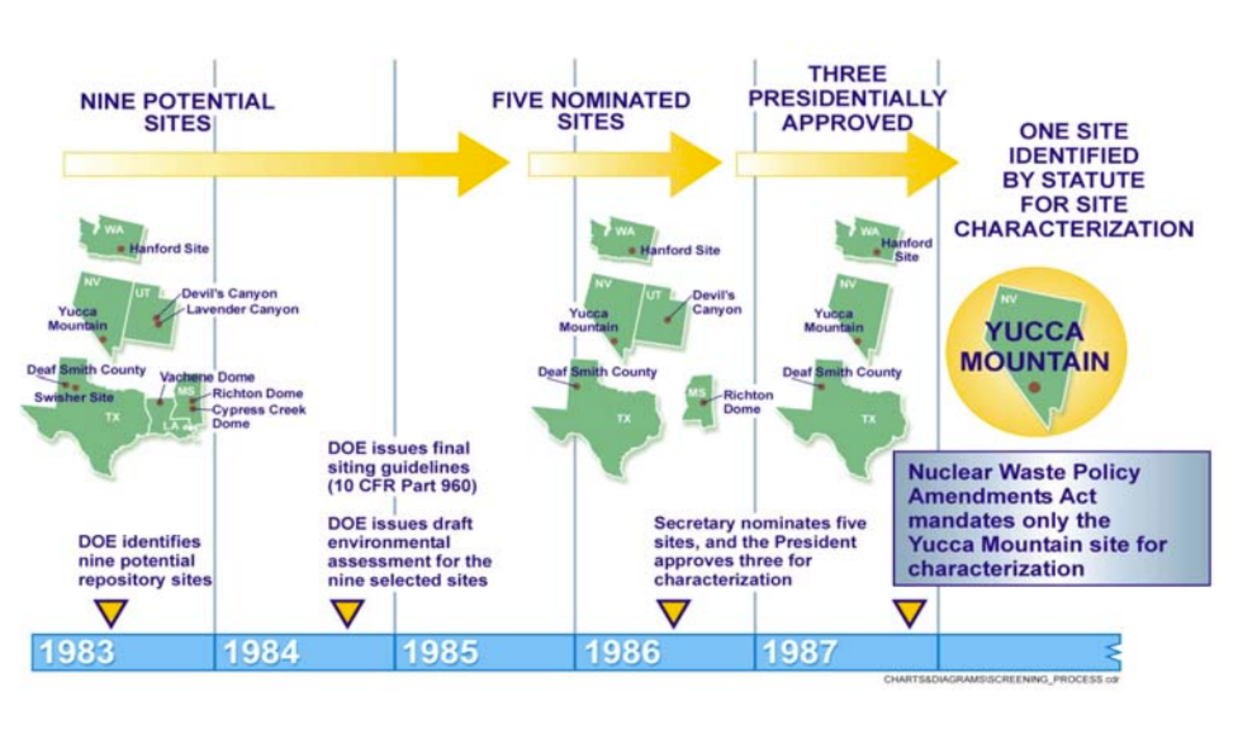
\includegraphics{nine_sites_to_one.eps}
  \end{center}
  \caption{The siting process began at nine sites and downselected to one 
    \cite{peters_what_2013}.}
  \label{fig:nine_sites_to_one}
\end{figure}

\end{frame}

%%--------------------------------%%
\begin{frame}[ctb!]
  \frametitle{Selection of Yucca Mountain}

  The Yucca Mountain Site was selected and accepted by the office of President 
  Ronal Reagan in 1987. Further spent fuel disposal R\&D would work toward a 
  lisence applicaton for the Yucca Mountain Site. 
  \begin{figure}[htbp!]
  \begin{center}
    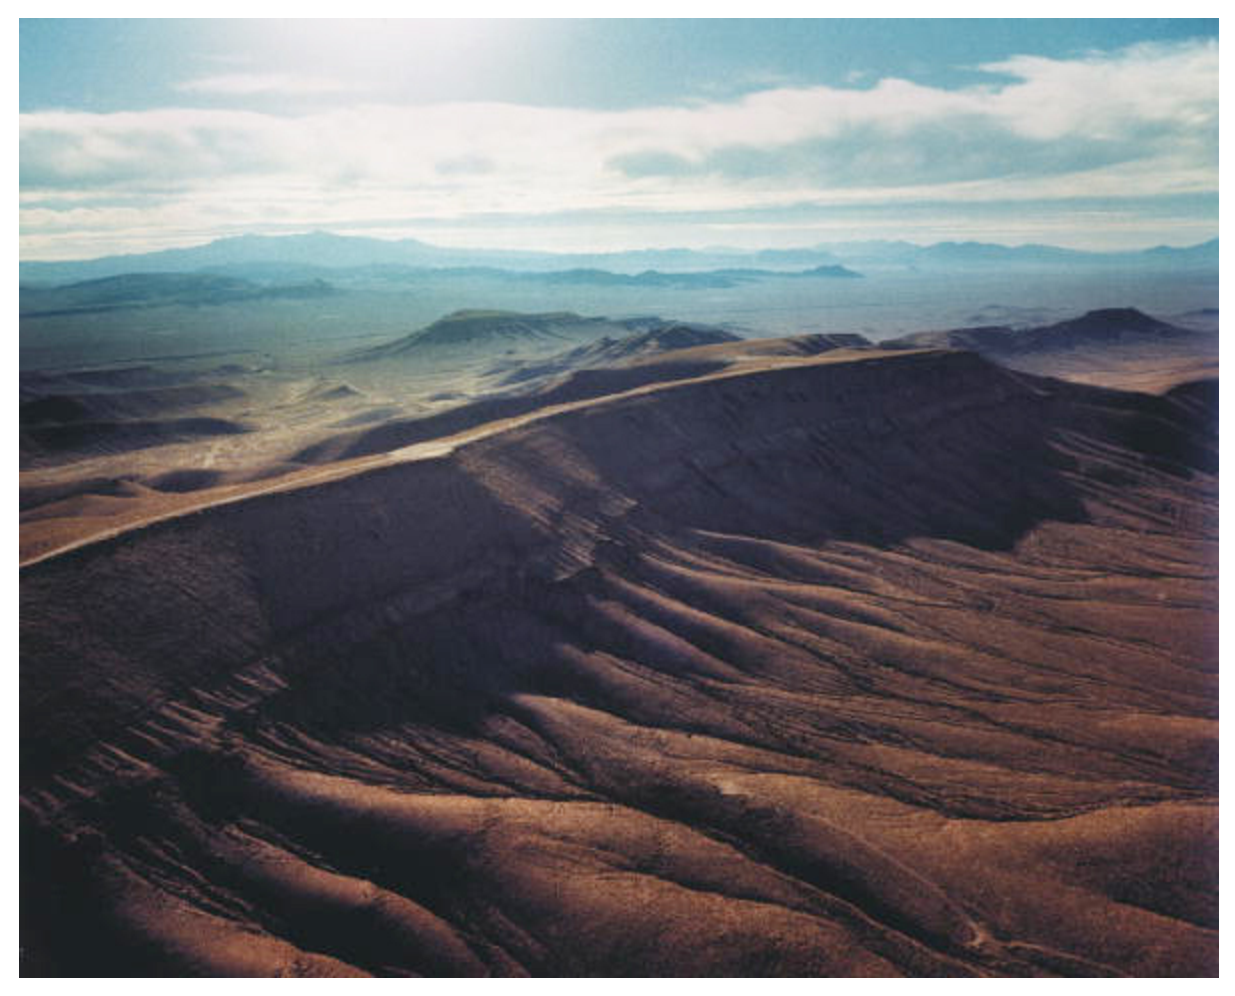
\includegraphics{yucca_site.eps}
  \end{center}
  \caption{Yucca Mountain in southern Nevada \cite{wherever_you_got_this}.}
  \label{fig:yucca_site}
\end{figure}

\end{frame}
